\chapter{Untersuchung der Messdaten}
Um eine Aussage über die Qualität des Touchscreen treffen zu können, werden mehrere Untersuchungen angestellt. 

Bei der ersten Untersuchung wurde auf die Mitte des Touchscreen gedrückt und die Position für eine gewisse Zeit gehalten.
Es wurden hierfür gefilterte und ungefilterte Messreihen erstellt (siehe Abschnitt \ref{ab:genau}).

Um die erste Untersuchung zu erweitern wurde die Mitte des Touchscreen, in der nächsten Untersuchung, wiederholt gedrückt. Hierbei ist die Wiederholbarkeit eines Punktes auf dem Touchscreen untersucht worden. 
Die Auswertung ist in Abschnitt \ref{ab:wiederholung} zu finden.

Bei der letzten Untersuchung wurde die Linearität des Touchscreen untersucht. Hierfür gibt der Hersteller eine Garantie, unter der sich die Linearität des Touchscreen befinden soll. 
Den Wert der angegeben wird liegt bei \SI{1,5}{\%} (siehe \ref{ds:touch} Seite 3 des Datenblatts). 

Um die Nachfolgende Untersuchungen korrekt durchführen zu können muss zu nächst der Reaktionsbereich des Touchscreens ermittelt werden.
Durch seine Bauform hat dies einen Randbereich an dem es nicht zuverlässig Werte ausgibt. Umkehrschluss, das Programm erkennt nicht das etwas den Touchscreen betätigt. 
Durch Untersuchungen des Randbereichs wurde in X-Richtung ein Arbeitsbereich von \SI{214,5}{mm} und in Y-Richtung eine Bereich von \SI{161,0}{mm} ermittelt.

Durch Ausprobieren wurden die maximal und minimal ADC-Werte in die jeweilige Richtung ebenfalls ermittelt. 
\begin{table}[ht!]
    \caption{maximal und minimal ADC-Werte}
    \begin{center}
        \begin{tabular}{ c |c| c }
                & x-Richtung & y-Richtung \\ \hline
         max. ADC-Werte & 961 & 917 \\  \hline
         min. ADC-Werte& 68 & 108 \\   
        \end{tabular}
    \end{center}   
\end{table}

Mit diesen Werten lässt sich Arbeitsbereich (in ADC-Werten) des Touchscreen in jede Richtung bestimmen.
\begin{align}
    ADC_{x,len} &= 1024 - 68 -(1024-961)\nonumber\\
    ADC_{x,len} &= 893\label{eq:adcxlen}\\
    ADC_{y,len} &= 1024-108-(1024-917)\nonumber\\
    ADC_{y,len} &= 809\label{eq:adcylen}
\end{align}
Mit diesen Werten (Gleichung \ref{eq:adcxlen} und Gleichung \ref{eq:adcylen}) können im Anschluss die Werte in das metrische System überführt werden und die Auflösung des Touchscreen bestimmt werden.
In x-Richtung ergibt sich eine Auflösung von \SI{0,240}{\frac{mm}{ADC}} und in y-Richtung \SI{0,199}{\frac{mm}{ADC}}.

Diese unterschiedliche Werte haben den Ursprung, dass die ADC-Werte sich in x-Richtung auf eine größere Distanz verteilen als in y-Richtung.

\section{Genauigkeit bei konstanten Koordinaten}
\label{ab:genau}
Bei dieser Untersuchung wurden zwei separate Messungen durchführen. Im ersten Durchlauf wurden die Werte mit dem Medianfilter verarbeitet, bevor sie ausgegeben wurden. Einen Ausschnitt der Messdaten ist in Tabelle \ref{tab:messgenaufilter} (siehe Seite \pageref{tab:messgenaufilter}) dem Bericht beigelegt.
Im zweiten Durchlauf wurden die direkten und ungefilterte Werte ausgegeben. Hierzu ist ebenfalls ein Ausschnitt der Messdaten beigefügt (siehe \ref{tab:messgenauunfilter} Seite \pageref{tab:messgenauunfilter}). 
In den Abbildungen \ref{fig:filtered} und \ref{fig:unfiltered} sind die Messdaten der x- und y-Komponenten aufgetragen (siehe Seite \pageref{fig:filtered}).

Die Auswertung der Messdaten ist in Tabelle \ref{tab:genaufilter} und \ref{tab:genauunfilter} zu finden.
Bei der Auswertung ist zu beachten das es um zwei separate Messreihen handelt. 
Die Messreihe der ungefilterten Werte weißt eine höhere Genauigkeit auf als die gefilterten Werte. Daraus lässt sich folgendes Ableiten. 
Zum einen ist das Messverfahren, der Rohdaten, gut umgesetzt und weißt eine hohe Präzision auf. Zum anderen gibt es ein Hinweis darauf, dass die eigens geschrieben Filterfunktion nicht akkurat arbeitet.



\begin{table}[ht!]
    \caption{Auswertung der gefilterten Messdaten }
    \begin{center}
        \begin{tabular}{ |c|c|c|c|c|c|c| }
          \hline&\multicolumn{2}{c|}{Median}& \multicolumn{2}{c|}{Standardabweichung}&\multicolumn{2}{c|}{Varianz} \\ \hline
         Einheit    &(ADC)              &mm             &(ADC)          &mm             &(ADC)      &mm\\\hline
         x-Richtung & \SI{499,0}{}      & \SI{119,861}{}&\SI{0,0}{}     &\SI{0,0}{}     &\SI{0,0}{} & \SI{0,0}{} \\  \hline
         y-Richtung & \SI{509,999}{}    & \SI{101,495}{}&\SI{0,049}{}   &\SI{0,010}{}   &\SI{0,0}{} & \SI{0,0}{} \\ \hline  
        \end{tabular}
        \label{tab:genaufilter}
    \end{center}   
    \caption{Auswertung der ungefilterten Messdaten}
    \begin{center}
        \begin{tabular}{ |c|c|c|c|c|c|c| }
          \hline&\multicolumn{2}{c|}{Median}& \multicolumn{2}{c|}{Standardabweichung}&\multicolumn{2}{c|}{Varianz} \\ \hline
          Einheit &(ADC)&mm&(ADC)&mm&(ADC)&mm\\\hline
          x-Richtung & \SI{499,0}{} & \SI{119,861}{}&\SI{0,0}{}&\SI{0,0}{}&\SI{0,0}{} & \SI{0,0}{} \\  \hline
          y-Richtung & \SI{510,0}{} & \SI{101,496}{}&\SI{0,0}{}&\SI{0,0}{}&\SI{0,0}{} & \SI{0,0}{} \\ \hline  
        \end{tabular}
        \label{tab:genauunfilter}
    \end{center}   
\end{table}


\begin{figure}[ht!]
    \centering
    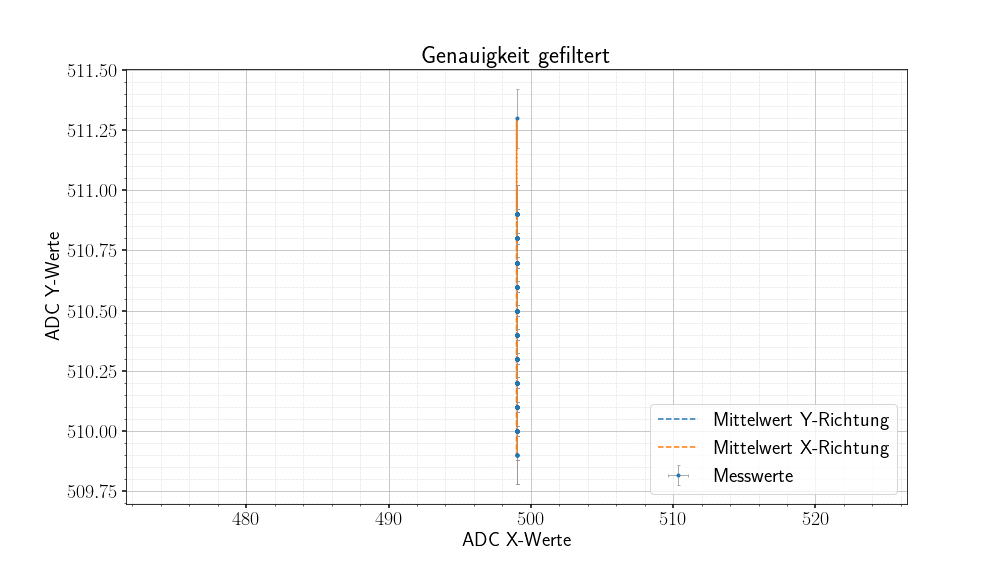
\includegraphics[width=\linewidth]{fig/filtered.png}
    \caption{Darstellung der gefilterten Messreihe}
    \label{fig:filtered}
    \centering
    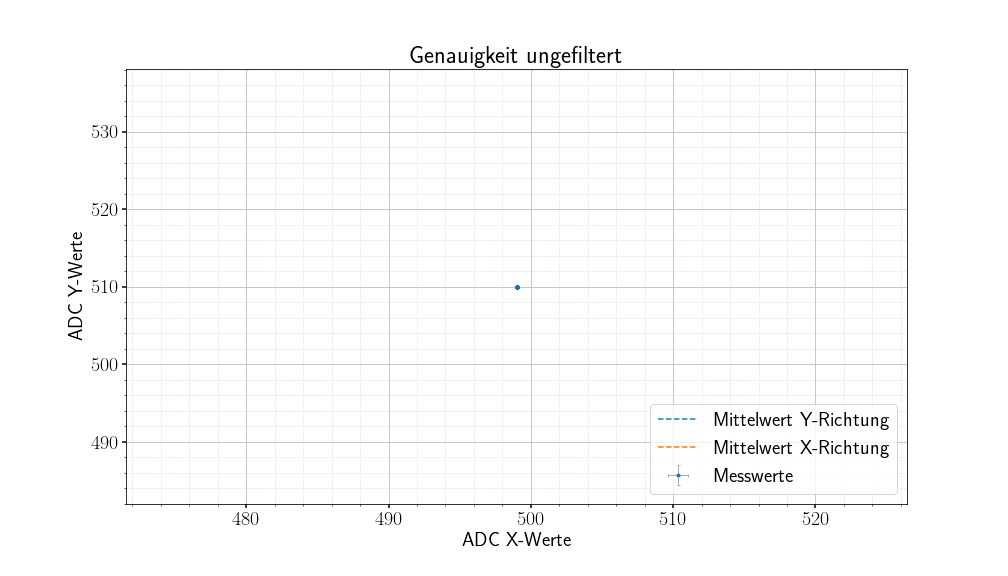
\includegraphics[width=\linewidth]{fig/unfiltered.png}
    \caption{Darstellung der ungefilterten Messreihe}
    \label{fig:unfiltered}
\end{figure}

\newpage

\section{Reproduzierbarkeit von Koordinaten}
\label{ab:wiederholung}
Um die Reproduzierbarkeit von Koordinaten zu untersuchen, wurde die Mitte des Touchscreen mehrmals berührt. Dabei wurden die ADC-Werte aufgezeichnet.
Ein Ausschnitt zu dieser Messreihe ist im Anhang auf Seite \pageref{tab:messwiederholung}. Die Messreihe wurde ebenfalls in einem Diagramm (Abb. \ref{fig:wiederholung} auf Seite \pageref{fig:wiederholung}) aufgetragen.

Die Auswertung der Messdaten sind in Tabelle \ref{tab:wiederholung} zu sehen. 
Diese zeigt, dass die Standardabweichung ähnlich der Auflösung. Dies lässt ebenfalls auf ein akkurat arbeitender Touchscreen schließen.


\begin{table}[ht!]
    \caption{Auswertung der Reproduzierbarkeit von Koordinaten}
    \begin{center}
        \begin{tabular}{ |c|c|c|c|c|c|c| }
          \hline  
         &\multicolumn{2}{c|}{Median}& \multicolumn{2}{c|}{Standardabweichung}&\multicolumn{2}{c|}{Varianz} \\ \hline
         Einheit    &(ADC)              &mm             &(ADC)          &mm             &(ADC)          &mm\\\hline
         x-Richtung & \SI{510,75}{}    & \SI{122,683}{}&\SI{0,894}{}   &\SI{0,215}{}   &\SI{0,8}{}     & \SI{0,192}{} \\  \hline
         y-Richtung & \SI{515,858}{}    & \SI{102,661}{}&\SI{1,159}{}   &\SI{0,231}{}   &\SI{1,3}{}     & \SI{0,259}{} \\ \hline  
        \end{tabular}
        \label{tab:wiederholung}
    \end{center}   
\end{table}


\begin{figure}[ht!]
    \centering
    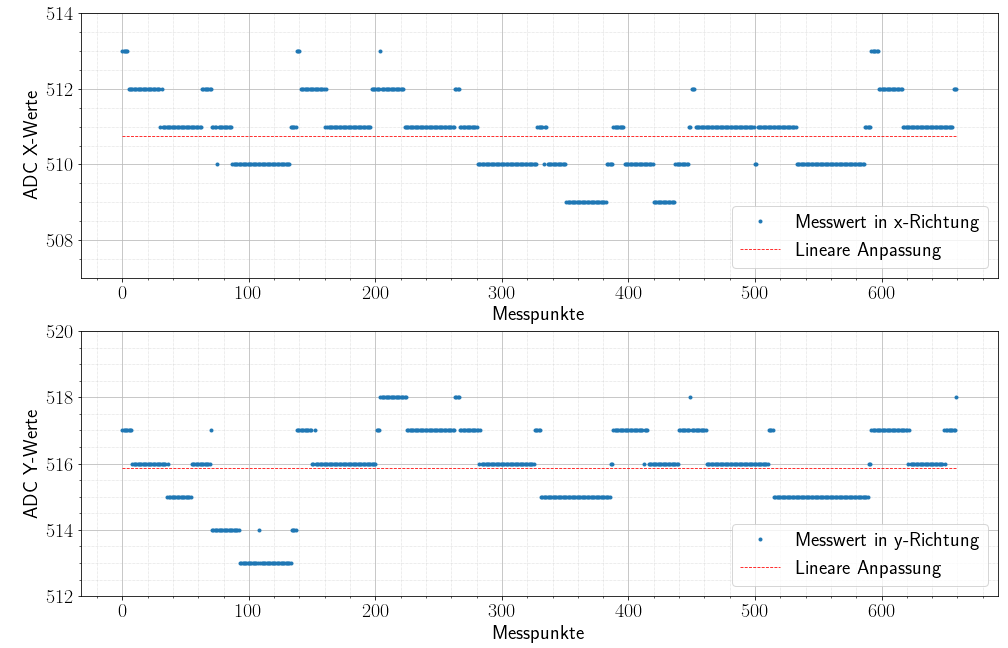
\includegraphics[width=\linewidth]{fig/wiederholung.png}
    \caption{Darstellung der Reproduzierbarkeit von Koordinaten}
    \label{fig:wiederholung}
\end{figure}
\section{Linearität in x- und y-Richtung}
\label{ab:linear}
Um eine Aussage über die Linearität des Touchscreens treffen zu können, wurden in x- und y-Richtung, auf dem Touchscreen alle \SI{10}{mm} eine Markierung gesetzt (siehe Abb. \ref{fig:messlinear}).

Die jeweilige Komponenten wurde anschließend jeweils über die physikalische Strecke in einem Diagramm dargestellt (siehe Abb. \ref{fig:xlinear} und Abb. \ref{fig:ylinear}). 
Die Messwerte wurden mittels einer linearen Anpassung anschließend ausgewertet (siehe Abb. \ref{fig:xfit} und Abb. \ref{fig:yfit}).

Das \(\chi^2\) gibt Auskunft darüber in welchem Maß Werte miteinander zusammenhängen. 
Je kleiner dieser Wert ist desto eher stimmt die Linearität überein. Bei der linearen Anpassung in x-Richtung wurde ein \(\chi^2\) von \(0,294\) ermittelt. Für die Linearität in y-Richtung wurde ein \(\chi^2\) von \(5,946\) ermittelt.

Bei der Untersuchung, der Linearität in y-Richtung, gibt es bei Abstand 40 mm ein Messpunkt der von der Messpunktewolke und der dazugehörigen linearen Anpassung abweicht. Dieser Messpunkt führt zu diesem größeren \(\chi^2\) als im Vergleich zur Messreihe  in x-Richtung.

Um Abschließend eine Aussage treffen zu können, ob diese Werte den Angaben des Datenblatts entsprechen (Anhang \ref{ds:touch}, Seite \pageref{ds:touch}), muss der Grenzwert der Chi-Quadrat-Verteilung mit den Werten der Linearen Anpassung verglichen werden.
Im Datenblatt wird eine Linearität von \SI{1,5}{\%} garantiert. In der Wertetabelle von \cite{papula} gibt es nur Grenzwerte für \SI{1}{\%} oder \SI{2,5}{\%}. Der gelistete Wert für zwei Freiheitsgrade und \SI{1}{\%} liegt bei 7,88.
Sowohl das \(\chi^2\) in x-Richtung wie auch in y-Richtung ist kleiner dieser Werte. Dies lässt darauf Schließen, dass dieser Touchscreen eine Linearität von unter \SI{1}{\%} aufweist.
\begin{figure}
    \begin{minipage}{0.49\linewidth}
        \centering
        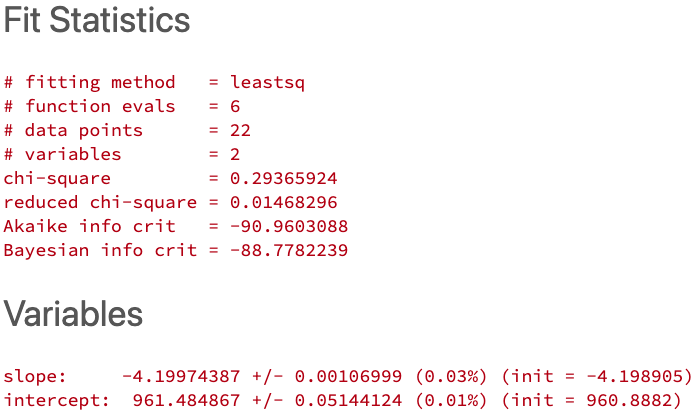
\includegraphics[width=\linewidth]{fig/xfit.png}
        \caption{Auswertung der Linearität in x-Richtung}
        \label{fig:xfit}
    \end{minipage}
    \begin{minipage}{0.49\linewidth}
        \centering
        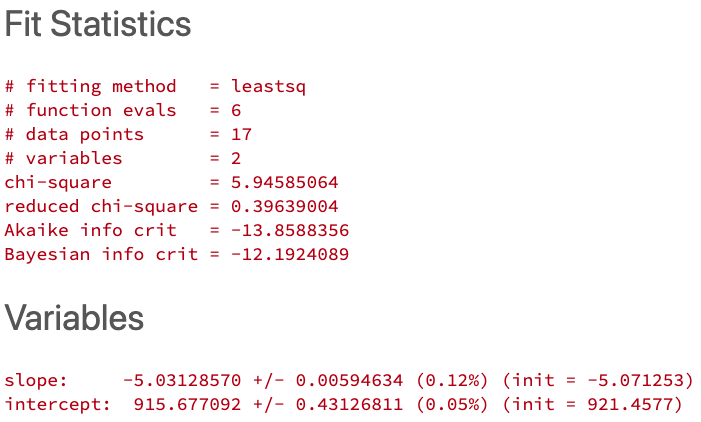
\includegraphics[width=\linewidth]{fig/yfit.png}
        \caption{Auswertung der Linearität in y-Richtung}
        \label{fig:yfit}
    \end{minipage}
\end{figure} 
\begin{figure}[ht!]
    \centering
    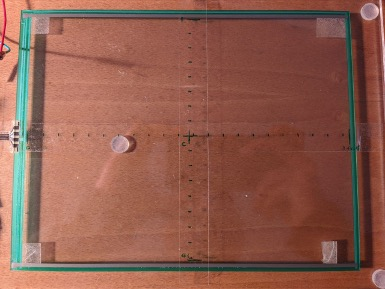
\includegraphics[width=0.6\linewidth]{fig/messlinear.jpg}
    \caption{Messaufbau für Linearität in x- und y-Richtung}
    \label{fig:messlinear}
\end{figure}

\begin{figure}[ht!]
    \centering
    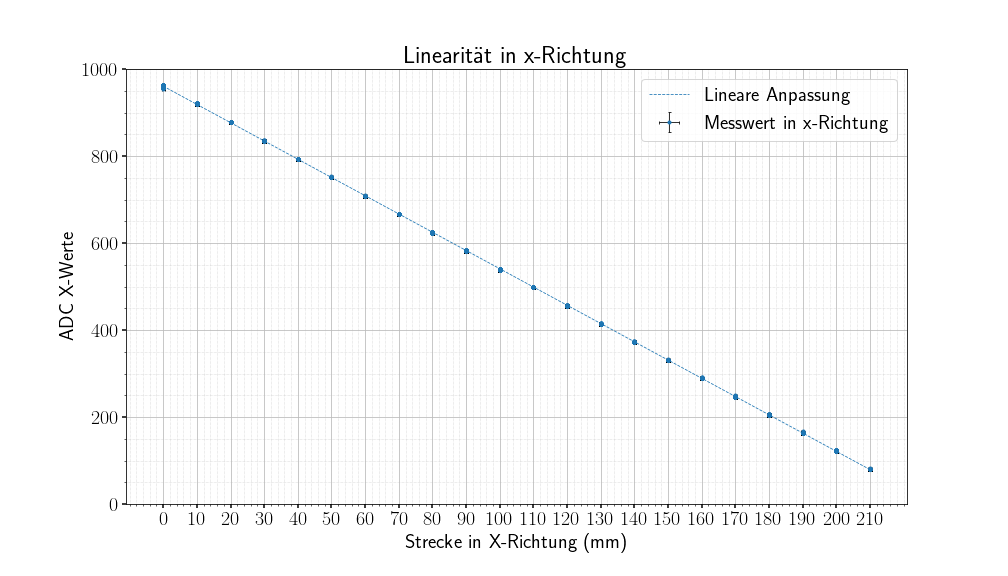
\includegraphics[width=\linewidth]{fig/8_linearitaet_x.png}
    \caption{}
    \label{fig:xlinear}
    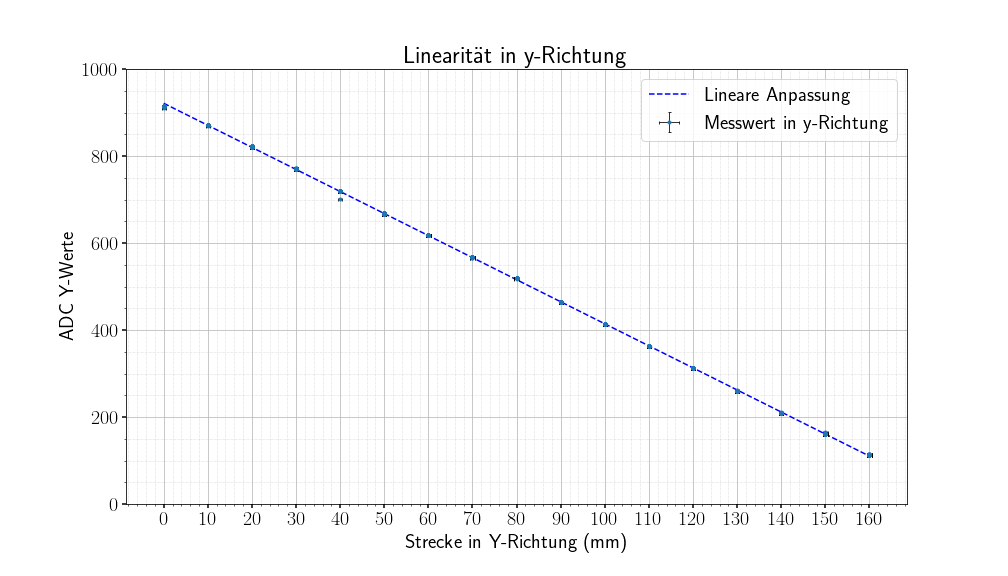
\includegraphics[width=\linewidth]{fig/8_linearitaet_y.png}
    \caption{}
    \label{fig:ylinear}
\end{figure}
